\documentclass[letterpaper,10pt,onecolumn,draftclsnofoot]{IEEEtran}
\usepackage{times}

\usepackage[english]{babel}
\usepackage[margin=0.75in]{geometry}
\usepackage{graphicx}

\DeclareGraphicsExtensions{.png}

\title{Object Velocity Tracking Requirements Document}
\author{Alex Bailey, Ben Wick, Dylan Washburne\\CS 461, Fall Term}

\begin{document}

\begin{titlepage}

\maketitle

\begin{abstract}
%Using a stationary camera, with the intent of being mounted on a car, we are attempting to  detect objects and determine the velocities of those objects relative to the Observer (camera).
Using a stationary camera, we are attempting to detect objects and determine the velocities of those objects relative to the Observer (camera).
This will be done by having the camera recognize a specific type of object, yet to be determined, in space and determine their velocities based on the rate at which they travel through the frame.
The speed of the objects will be displayed on a computer application window.
%If the camera is on a moving object, then we will need to either have a way for the product to measure it's own velocity, likely with an accelerometer or connect to the object, if the object is measuring it's own velocity.
To make this work, we will have to research the varieties of cameras available to use, as well as the API’s they operate with.
%We will also have to review the available computer vision software and determine which is the most appropriate for our needs.
We will review the available computer vision software and determine which is the most appropriate for our needs.
We will also design a computer application that will be the user interface for the product.
%From this, we will determine the best camera to be used and from there create a object tracking program.
From these we will create an object tracking program that will not have the shortcomings of the current object tracking methods, such as being only able to track one object and having trouble in the rain.

 
\end{abstract}

\end{titlepage}


%Beginning of introduction
\section{Introduction}
\subsection{Purpose}
The purpose of this document is to present a detailed description of the requirements for the "Video Radar" software.
This document is intended for the main use of the client, as well as the professor and the teacher assistants and will be proposed to the client for its approval.

\subsection{Scope}
Our product, the "Video Radar", will be able to identify a specific type of object, such as a person or a car, calculate the object's velocity, then display the velocity on the screen.
Our product will be beneficial over other products in that it can function unmanned, will specify which target is being tracked, and will be able to track multiple objects.
\subsection{Definitions, acronyms, and abbreviations}
\begin{tabular}{|p{4cm}|p{12cm}|}
	\hline
	\textbf{Term} & \textbf{Definition} \\
	\hline
	API (Application program interface) & A particular set of rules and specifications that software programs can follow to communicate with each other. \\
	\hline
	User & Someone who is interacting with the software. \\
	\hline
	Object & The entity being tracked by the video feed.  \\
	\hline
	
\end{tabular}



\subsection{Overview}
The rest of the document contains two additional sections.
The first section is the overall description.
This section will describe the intended use of the software and give background.
The last section is the specific requirements section.
This section contains all the software requirements.

%Beginning of overall desciption
\section{Overall description}
\subsection{Product perspective}
Our product is a self-contained product. 
Our product's interface will consist of a window where the user can activate the camera and velocity tracking.
There will be a menu bar in the application that will allow the user to specify aspects of the product, as shown by Section C in the picture A below.
Our products application window will consist of a small button row at the bottom for essential buttons, such as the start and stop buttons, as depicted in Section B of picture A below.
The application will have a central section for displaying the video captured by the camera with our information overlay, such as Section A of picture A below.
We will be using computer vision software in order to identify the type of object and track its location across the frame.
The product will have only one mode of operation, the on mode, where the product constantly processes the images from the camera and velocity is displayed.
This mode requires no input from the user except to turn off.
The camera will not have any automated motion.
The user will have to manually adjust the camera.
The camera will have a fixed zoom that the user will not be able to change.

\begin{figure}[h]
    \centering
    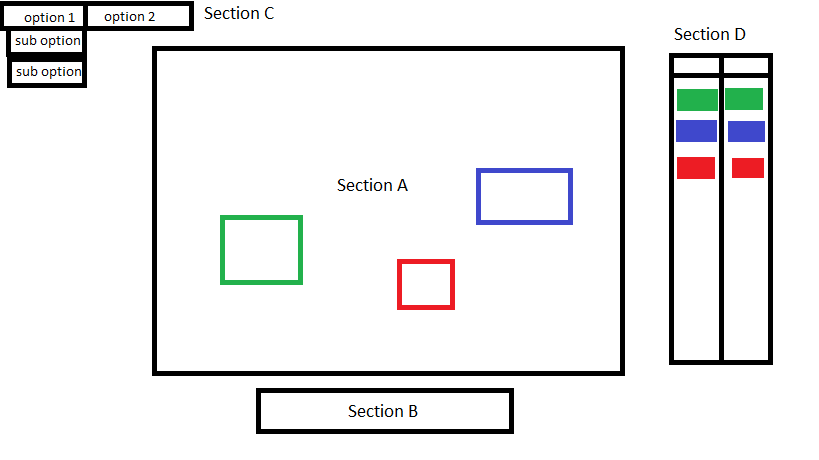
\includegraphics[scale=0.75]{cs_461_mock_up}
    \caption{Picture A: Mock up of Application window}
    \label{fig: pic_a}
\end{figure}


\subsection{Product functions}
The software will be connected to a camera with a live video feed.
It will then be able to detect objects that are specified for the users needs.
The software will than be able to acquire the velocity at which the objects are traveling.
%This information will be stored into a table for the user to see.


\subsection{User characteristics}
This software is intended to be used by many different users.
The types of users are broken down into two categories: users who wish to track cars, users who wish to track people.
These users have different use for the product but the software should work the same way for both users.

Users who wish to track cars may use the product to detect the velocity of a moving car on the road.
This means the user will set the stationary camera and point it in the direction of moving vehicles to obtain the velocity.

Users who wish to track the velocity of people may also use the product.
These users will follow the same procedure as the other users but instead, the software will detect the velocity of people.

\subsection{Constraints}
This product will likely require a nontrivial amount of resources to perform its task at the constant interval we require.
As a result, our product will either need to come with a dedicated computer to do the processing, or it will have to interface with existing computers which we expect to be in the locations of use.

In accordance with federal laws, the camera is allowed to be recording anything described as "within plain sight".
The proper use of this falls on the user, and must be disclaimed before use.

The product's reliability of use can be described in a number of ways.
The camera should be recording at a constant and stable rate.
The objects in the scene should be properly identified with 70\% accuracy.
The tracking of an identified object's velocity should be within 90\% of the objects actual velocity.
The velocity tracking should also be reliably given every 0.5 seconds, without any notable dips in rate of recording and processing.

While the video recorded is protected by federal laws, the information nonetheless must meet certain security standards.
If the video data is to be saved locally, it should also respect encryption of the product it is saved on.
Should the video be live streamed to a remote location, it must enter a stable connection to deliver to the intended viewer.

\subsection{Assumptions and dependencies}
We assume that if our products camera needs to move that our product would be able to either handle the motion of the camera and still be able to track velocities or be mounted securely enough to minimize motion of the camera, allowing the product to track velocities.
We assume that the computer vision software will be able to recognize an object within enough time after entering the frame so that there will be enough time for the velocity algorithm to calculate the velocity.

%Beginning of specific requirments
\section{Specific requirements}
%I don't know about the "cross-reference" part, I'm just ignoring that for now
The product must be able to identify objects in frame, and differentiate them from the background.
%The product must identify desired objects at least 70\% of the time while they are in frame.
When the product identifies an object as the desired type, at least 70\% of the time this must actually be the desired object type.

The product must be able to track the velocities of identified objects.
For each object identified in the scene, the velocity the program displays to the user must be within 90\% of the objects true velocity.

The product must have the capability to identify and track multiple objects simultaneously.
%It must be able to track as many objects as it can identify, however we would like the product to be able to identify up to 6 objects at once under most setup conditions. 
It must be able to identify and track at least 4 objects simultaneously.
At the same time, should the proper conditions present themselves, the product should be able to automatically identify as many objects it can locate in frame, should that number exceed 4.

%Parallel and perpinduicular
The product should be able to perform its velocity analysis on objects that are moving in various directions.
While it should track the velocities of objects moving perpindicular to the camera, it should also be able to identify the velocities of objects moving parallel to the camera, or at any variation in between.
The velocities returned are within 90\% as stated above, however direction should not cause the product to fail its purpose.

%Max effective view distance of 100m
The product will accurately work within 100m of the camera's placement.
Objects within 100m of the camera's placement, within its view angle and with an unobstructed line of sight, should all be able to be identified by the camera, reflecting the accuracy requirements described above.
Objects beyond the maximum effective range can potentially still be identified if the conditions allow, but are not granted the same accuracy guaranty.

\end{document}